\newpage{\ } 
\thispagestyle{empty} 

\chapter{Pruebas experimentales}
\lhead{Capítulo 5. \emph{Pruebas experimentales}} % This is for the header on each page - perhaps a shortened title
En este capítulo se menciona las métricas de evaluación utilizadas para medir el desempeño de la metodología propuesta. Por otro lado, se detallan los experimentos realizados y los  resultados tanto de la metodología propuesta y  del estado del arte, seguidamente se esboza la comparación y la posterior discusión de los mismos.


\section{Métricas de evaluación}

Como se había mencionado anteriormente, un diagnóstico consiste en determinar la presencia o ausencia de una enfermedad, para este caso particular es la  presencia o ausencia de la retinopatía diabética. Un diagnóstico positivo determina la presencia de retinopatía diabética y un diagnóstico negativo determina la ausencia de la misma.

Dado un clasificador y un diagnóstico, hay cuatro resultados posibles. Si el diagnóstico es positivo y se clasifica como positivo, se cuenta como un verdadero positivo (VP); si se clasifica como negativo, se cuenta como un falso negativo (FN). Si el diagnóstico es negativo y se clasifica como negativo, se cuenta como un verdadero negativo (VN); si se clasifica como positivo, se cuenta como un falso positivo (FP) \cite{fawcett2006introduction}. En la FIGURA \ref{fig:clasificacion} se puede ver la gráfica de una matriz en donde se ve los cuatro casos posibles del par diagnóstico y clasificación. 
%Las limitaciones de la precisión de diagnóstico como una medida del desempeño de decisión, requiere la introducción de los conceptos de sensibilidad y especificidad de una prueba diagnóstica \cite{metz1978basic,fawcett2006introduction}.

\begin{figure}
	\centering
		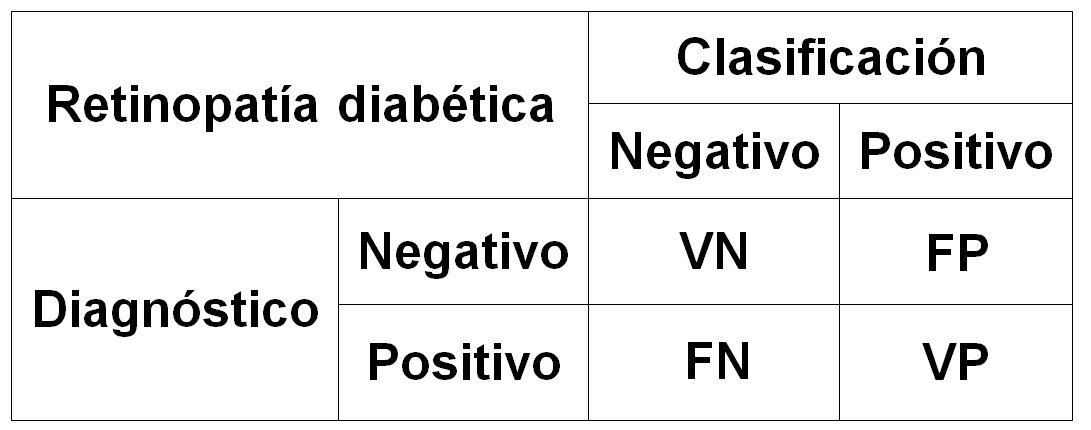
\includegraphics[width=0.65	\textwidth]{./Figures/cap5/matrizd.PNG}
	\caption{Esquema de clasificación.}

	\label{fig:clasificacion}
\end{figure}

Para evaluar los resultados obtenidos se hace uso de las siguientes métricas de evaluación: sensibilidad, especificidad y exactitud. A continuación las mismas se explican con más detalles.  
\subsection{Sensibilidad}
Es la probabilidad de clasificar correctamente a un paciente con retinopatía diabética, es decir, la probabilidad de que  un paciente con retinopatía diabética sea diagnosticado con resultado positivo. La sensibilidad es, por lo tanto, la capacidad para detectar pacientes con retinopatía diabética \cite{pita2003pruebas}.

\begin{equation}
\label{eq:sensibilidad}
\small	Sensibilidad=\frac{\text{VP}}{\text{VP} + \text{FN}}
\end{equation}

\subsection{Especificidad}
Es la probabilidad de clasificar correctamente a un paciente sin retinopatía diabética, es decir, la probabilidad de que para un sujeto sano se obtenga un resultado negativo. En otras palabras, se puede definir la especificidad como la capacidad para detectar pacientes sin retinopatía diabética \cite{pita2003pruebas}. 
\begin{equation}
\label{eq:especificidad}
\small	Especificidad=\frac{\text{VN}}{\text{VN} + \text{FP}}
\end{equation}

\subsection{Exactitud}
Es la probabilidad de clasificar correctamente a un paciente, dicho de otra manera, la probabilidad de que un paciente sano o enfermo obtenga un diagnóstico correcto. En otras palabras, se puede definir la exactitud como la capacidad para detectar pacientes con o sin  retinopatía diabética \cite{pita2003pruebas}. 
\begin{equation}
\label{eq:exactitud}
\small	Exactitud = \frac{VN + VP}{VN + FP + FN + VP}
\end{equation}

\section{Pruebas y resultados experimentales}
En esta sección  se profundiza el trabajo base del estado del arte, motivo por el cual fue seleccionado y sus resultados. Igualmente  se exponen los resultados obtenidos por nuestra metodología y se realiza una comparación con respecto a las métricas de evaluación.

\subsection{Base de imágenes MESSIDOR}
Para las pruebas se utiliza la base de imágenes pública MESSIDOR  \cite{messidor}. Estas imágenes poseen una resolución de 2240 x 1488 píxeles. Las imágenes seleccionadas para las pruebas incluyen imágenes borrosas y con poca iluminación con el fin de probar la robustez del detector.

\subsection{Metodología del trabajo base}
Selvathi et al. \cite{selvathi2012automated} proponen un sistema  de detección automática de retinopatía diabética a partir de imágenes de retina, cuyo trabajo se compara con nuestra metodología propuesta.
Las razones por las cuales este trabajo fue seleccionado, se basa en las siguientes similitudes:
\begin{itemize}
\item Utilizaron segmentaciones de vasos sanguíneos, exudados duros y microaneurismas.
\item Utilizaron  una base de imágenes pública MESSIDOR \cite{messidor} con imágenes de retina previamente diagnosticada por profesionales médicos.
\item Estructuraron su metodología en tres módulos, el primero de ellos el de detección y segmentación, luego el módulo de extracción de características y por último el módulo de clasificación. 
\item Hicieron uso del clasificador binario SVM.
\item Es el trabajo con mejores resultados para el diagnóstico automatizado de presencia o ausencia de retinopatía diabética para la base de imágenes de MESSIDOR  \cite{messidor}.
\end{itemize}

Además de estas semejanzas, en \cite{selvathi2012automated} los resultados reportados indican que el enfoque de Selvathi et al. es el más promisorio, por tal motivo, es el fundamento principal de la comparación con este trabajo.


%la propuesta de este trabajo  base a la etapa de investigación se concluye que ellos obtuvieron los mejores resultados en  el diagnóstico de la retinopatía diabética en relación a otros similares, lo que representa el fundamento principal de la comparación con este trabajo.
\subsubsection{Resultados del estado del arte}
Selvathi et al. \cite{selvathi2012automated} utilizaron 200 imágenes para sus experimentaciones de las cuales  50 fueron  imágenes de entrenamiento, 25 imágenes sin retinopatía diabética y 25 imágenes con retinopatía diabética. 
En la etapa de pruebas emplearon 150 imágenes, 75 imágenes con retinopatía diabética y 75 imágenes sin retinopatía diabética, diagnosticadas por el clasificador binario SVM.

De las 75 imágenes con retinopatía diabética, 4 no fueron clasificadas correctamente, dando una tasa de sensibilidad 94,67\%, mientras que 7 de 75 imágenes sin retinopatía diabética fueron mal diagnosticadas, teniendo así una tasa de especificidad del 90,67\%, para dar  un total de 139 imágenes correctamente diagnosticada de 150 imágenes de prueba logrando una tasa de exactitud del 92,67\%.

Los resultados  obtenidos por \cite{selvathi2012automated} se pueden apreciar en la TABLA \ref{tab:resultados1}. 

\begin{table}[!hbtp]
\begin{center}
\caption{Resultados de Clasificación de Selvathi 2012 \cite{selvathi2012automated}.}
\resizebox{15cm}{!} {
\begin{tabular}{|p{2.2cm}|p{1.9cm}|p{2.2cm}|p{2.4cm}|p{2cm}|}


\hline
Métricas &  Imágenes de entrenamiento & Imágenes de prueba  & Imágenes clasificadas correctamente  & Tasa \\ 
\hline
Sensibilidad & 25 & 75 & 71 & 94,67 \\
Especificidad & 25 & 75 & 68 & 90,67  \\
Exactitud  & 50 & 150  & 139  & 92.67 \\
%\hlineExactitud  & 50 & 150  & 139  & 93 \\
\hline
\end{tabular}
}

\label{tab:resultados1}
\end{center}
\end{table}
 
\subsection{Prueba experimental I}
Para los experimentos se hace uso de 200 imágenes de la base pública MESSIDOR. El software utilizado para la implementación de los módulos fue el \textit{toolbox} de procesamiento de imágenes de MATLAB versión 2013b. El primer paso a realizarse es la segmentación de los vasos sanguíneos, exudados duros y microaneurismas. Luego se realiza la extracción de características en base a las imágenes segmentadas. Por último, la clasificación y los resultados obtenidos  se exponen a continuación:

% 0.969333 0.952  0.9866667

\begin{table}[!hbtp]
\begin{center}
\caption{Resultados de Clasificación.}
\resizebox{15cm}{!} {
\begin{tabular}{|p{2.2cm}|p{1.9cm}|p{2.2cm}|p{2.4cm}|p{2cm}|}

\hline
Métricas &  Imágenes de entrenamiento & Imágenes de prueba  & Imágenes clasificadas correctamente  & Tasa \\ 
\hline
Sensibilidad & 25 & 75 & 71 & 94,67 \\
Especificidad & 25 & 75 & 74 & 98,67  \\
%\hline
Exactitud  & 50 & 150  & 145  & 96,67\\
\hline
\end{tabular}
}

\label{tab:resultados}
\end{center}
\end{table}


En la TABLA \ref{tab:resultados}, como se puede observar, se hace uso de 50 imágenes de entrenamiento que se seleccionaron aleatoriamente de un grupo de imágenes de entrenamiento, 25 imágenes sin retinopatía diabética y 25 imágenes con retinopatía diabética. Para probar el sistema se utiliza 150 imágenes de prueba, 75 imágenes con retinopatía diabética y 75 imágenes sin retinopatía diabética.

 Con respecto a los resultados obtenidos de las 75 imágenes con retinopatía diabética, 4 no fueron clasificadas correctamente, dando una tasa de sensibilidad 94,67\%, mientras que 74  de las 75 imágenes sin retinopatía diabética fueron diagnosticadas correctamente, es decir una tasa de especificidad de 98,67\%, para dar un total de 145 imágenes correctamente diagnosticadas de 150 imágenes de prueba logrando una tasa de exactitud del 96,67\%.


% Selvathi, D., N. B. Prakash, and Neethi Balagopal \cite{selvathi2012automated}.
%\begin{itemize}
%\item 200 imágenes: 100 normales, 100 con retinopatía diabética.
%\item Sensibilidad: 95\%.
%\item Especificidad: 91\%.
%\item Exactitud: 93\%.
%\end{itemize}
%\subsection{}


\subsection{Comparación y discusión de resultados}
% \cite{selvathi2012automated}
 En la TABLA \ref{tab:comparacion} se puede ver la comparación de los resultados y del estado del arte:
 \begin{table}[!hbtp]
 \caption{Comparación de clasificación.}
\begin{center}
\resizebox{15cm}{!} {

\begin{tabular}{|p{3.5cm}|p{2cm}|p{2cm}|p{2cm}|p{2cm}|p{2cm}| p{2cm}}
\hline
 &  Imágenes de entrenamiento &  Imágenes de Prueba & Sensibilidad & Especificidad & Exactitud   \\ 
 
\hline
Selvathi 2012 & 50 & 150& 94,67 & 90,67 & 92,67  \\
Método propuesto& 50 & 150 & 94,67 & 98,67 & 96,67   \\
\hline
\end{tabular}
}

\label{tab:comparacion}
\end{center}
\end{table}


Se puede apreciar que el método propuesto ha superado en especificidad e igualado en sensibilidad al propuesto por Selvathi et al. \cite{selvathi2012automated} obteniendo así mayor exactitud. 
  En el proceso de entrenamiento del clasificador, se emplea la misma cantidad de imágenes, de igual manera, se obtiene una mejora con respecto a las métricas: especificidad y exactitud.


El segundo experimento denota los valores de exactitud obtenidos en base a cierta cantidad de imágenes de entrenamiento.
\subsection{Prueba experimental II}
Para el segundo experimento, se usan 200 imágenes de la base de imágenes MESSIDOR, se toman 100 imágenes de entrenamiento y 100 imágenes de prueba.
El experimento consiste en tomar aleatoriamente $v$ imágenes de entrenamiento y hallar la exactitud obtenida al clasificar las 100 imágenes de prueba. Esto se realiza en 10 iteraciones. Luego, este procedimiento se repite para valores de $v=\{10,20,30,40,50,60,70,80\}$.

 \begin{figure}[H]
	\centering
		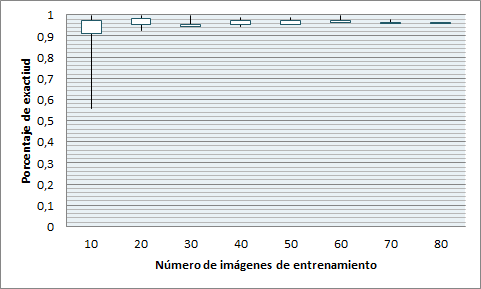
\includegraphics[width=0.65	\textwidth]{./Figures/cap5/boxplot.png}
	\caption{Diagrama de caja de los valores de exactitud obtenidos.}

	\label{fig:bp}
\end{figure}

En la FIGURA \ref{fig:bp} se puede ver que para menores cantidades de entrenamiento se obtuvieron resultados altos tanto como resultados bajos, es decir se tienen resultados inestables. A medida que fue aumentando la cantidad de imágenes de entrenamiento los resultados obtenidos se estabilizaron.

 \begin{figure}[H]
	\centering
		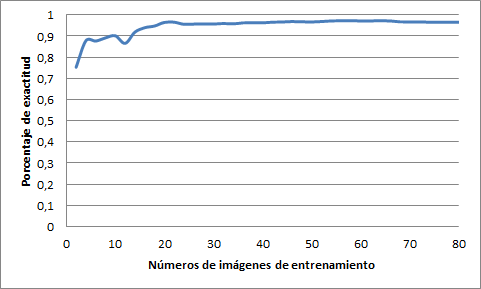
\includegraphics[width=0.65	\textwidth]{./Figures/cap5/exacTra.png}
	\caption{Porcentaje de exactitud por imágenes de entrenamiento.}

	\label{fig:exacNtrta}
\end{figure}
 


En la FIGURA \ref{fig:exacNtrta} se puede ver la curva generada por los valores de exactitud obtenidos en promedio de las 10 iteraciones para la clasificación en función de la imágenes de entrenamiento.
Se puede notar en la gráfica que por más de que aumente la cantidad de imágenes de entrenamiento la exactitud en la clasificación ya no se mejora.



%\section{Discusión de resultados}
   
 % Entre las características utilizadas en la detección de retinopatía diabética, la de mayor relevancia fueron los microaneurismas  debido a que su presencia o ausencia en la imagen de retina fue determinante en el diagnóstico realizado \cite{veritticlose} por el clasificador SVM.
  
\subsection{Dificultades encontradas} 
 Debido a la mala calidad de algunas imágenes se hace necesario evaluar automáticamente la calidad de las imágenes de retina para aumentar la exactitud en la detección de estructuras y patologías de la retina para un sistema de detección basado en técnicas de visión por  computadora. Una imagen se considera de mala calidad cuando es difícil o imposible hacer un  juicio clínico confiable con respecto a la presencia o ausencia de retinopatía diabética en la imagen \cite{niemeijer2006image}.  

 En la FIGURA \ref{fig:badQuality} se muestra una de las imágenes de mala calidad utilizada como imagen de prueba, en ella se puede notar poca iluminación debido al pequeño tamaño de la pupila y pérdida de contraste por el movimiento del ojo.
 
 \begin{figure}[H]
	\centering
		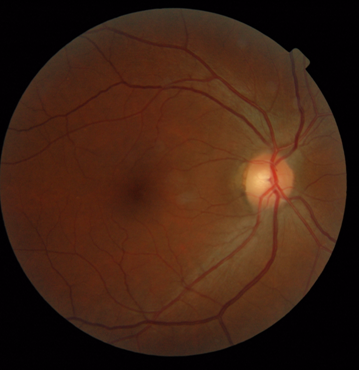
\includegraphics[width=0.65	\textwidth]{./Figures/cap5/badQ.png}
	\caption{Imágen digital de mala calidad.}

	\label{fig:badQuality}
\end{figure}
 



 
%Durante el proceso de desarrollo se comprobó que existe una relación  de costo entre la sensibilidad  y la especificidad del método, las mismas son inversamente proporcionales, lo que significa que a medida que aumenta la sensibilidad, la especificidad disminuye y viceversa. \cite{parikh2008understanding}.
Teniendo en cuenta los resultados favorables en base a los objetivos propuestos, en el siguiente y último capítulo se exponen las conclusiones de este trabajo  y finalmente trabajos futuros que puedan dar continuidad a este trabajo final de grado.